\documentclass[letterpaper]{article}

\usepackage{aaai2026}
\usepackage{times}
\usepackage{helvet}
\usepackage{courier}
\usepackage[hyphens]{url}
\usepackage{graphicx}
\usepackage{natbib}
\usepackage{caption}
\usepackage{amsmath}
\usepackage{amssymb}
\usepackage{booktabs}
\usepackage{multirow}
\usepackage{algorithm}
\usepackage{algorithmic}
\usepackage{tikz}
\usetikzlibrary{arrows.meta}

\urlstyle{rm}
\def\UrlFont{\rm}
\frenchspacing
\setlength{\pdfpagewidth}{8.5in}
\setlength{\pdfpageheight}{11in}
\setcounter{secnumdepth}{0}
\setlength{\textfloatsep}{6pt plus 1pt minus 1pt}
\setlength{\floatsep}{6pt plus 1pt minus 1pt}
\setlength{\intextsep}{6pt plus 1pt minus 1pt}

\pdfinfo{/TemplateVersion (2026.1)}

\title{Evaluating Counterfactual Explanations with Deterministic Heuristics and LLM-Based Review}

\author{
    AFRA Lama,
    MORTADA Daniel,
    RIABICHEFF Ivan,
    DESOIL Theo
}

\affiliations{
    Universit\'e Libre de Bruxelles\\
    INFO-H512 Current Trends of Artificial Intelligence\\
    \{lama.afra, daniel.mortada, ivan.riabicheff, theo.desoil\}@ulb.be
}

\begin{document}
\maketitle
\thispagestyle{plain}
\pagestyle{plain}

\begin{abstract}
Counterfactual explanations are attractive because they translate model decisions into actionable ``what would need to change'' statements. However, standard counterfactual metrics such as validity, proximity, sparsity, and diversity do not by themselves determine whether the proposed changes are plausible, actionable, or fair. We implement an end-to-end evaluation pipeline for DiCE counterfactuals on the Adult Income dataset. The pipeline trains a Logistic Regression classifier, generates DiCE counterfactuals for ten unfavourable predictions, evaluates them with two deterministic layers --- quantitative metrics and domain heuristics --- and then compares LLM-based evaluators against that structured evidence. In Phase 1, we implemented both a single-LLM evaluator and a multi-agent debate architecture; the debate was runnable but less reliable and more costly than the simpler baselines. In Phase 2, we reframed the task as substitution feasibility: can a calibrated single LLM approximate the metrics-only reference system while adding human-readable explanations? Calibration improved issue-label recall from 84\% to 96\% and exact issue-set match from 60\% to 90\% at 100\% precision; the optional explanation layer preserved 96\% recall while producing non-expert rationales at a higher (but still negligible) cost.
\end{abstract}

\section{Related Work and Problem Framing}
Counterfactual explanations answer a practical question: what minimal change to an input would have flipped a model's decision? \citet{wachter2017counterfactual} formalised them as a way to explain automated decisions without exposing model internals --- instead of reporting which coefficients mattered, a system states which input attributes would have produced a different outcome. This user-facing form is what makes counterfactuals attractive for explainable AI: in income prediction, a person classified as earning at most \$50K can be shown which feature changes would move the classifier to predict income above \$50K.

The difficulty is that a counterfactual can be valid for the classifier yet weak as advice. It may edit many attributes at once, touch protected or non-actionable features, propose temporally impossible changes (e.g.\ more education with no added years of age), or land just past the decision boundary so that a small perturbation flips it back. Work on algorithmic recourse therefore emphasises feasibility and actionability: a useful counterfactual must describe changes a person could plausibly make, not merely changes that satisfy the model \citep{karimi2021algorithmic}. DiCE, the generator we use, addresses part of this by producing a \emph{diverse set} of counterfactuals optimised for validity, proximity, sparsity, and diversity \citep{mothilal2020explaining}, and graph-based methods such as FACE enforce feasible paths along the data manifold \citep{poyiadzi2020face}. The common thread is that these objectives are necessary but not sufficient: a counterfactual set can be numerically diverse and proximal while still recommending implausible or unfair interventions, because recourse quality depends on domain constraints that the standard metrics do not encode.

This gap motivates our research question: \emph{how can DiCE-generated counterfactuals be evaluated beyond standard numerical metrics, and can LLM-based evaluators substitute or complement a deterministic, policy-grounded reference?} The project connects two seminar themes --- counterfactual explanations as an XAI method, and GenAI orchestration --- by defining one shared, structured case representation and running three evaluators over it (Fig.~\ref{fig:pipeline}): a deterministic heuristic baseline, a single LLM, and a four-role adversarial debate. We deliberately treat LLM evaluation as an empirical question rather than an assumption. The work has two phases. \textbf{Phase 1} compares the three architectures against a team-drafted reference and yields a negative result for the debate. \textbf{Phase 2}, prompted by an internal methodology critique, reframes the task as \emph{substitution feasibility}: instead of asking whether LLMs beat rules, we ask how closely, and at what cost, a calibrated LLM can reproduce the deterministic reference while adding human-readable explanations. The contribution is therefore not that LLMs universally replace rules, but a delimited account of when rules are preferable, when an LLM can approximate them, and where LLM explanations add interpretive value.

\begin{figure*}[t]
\centering
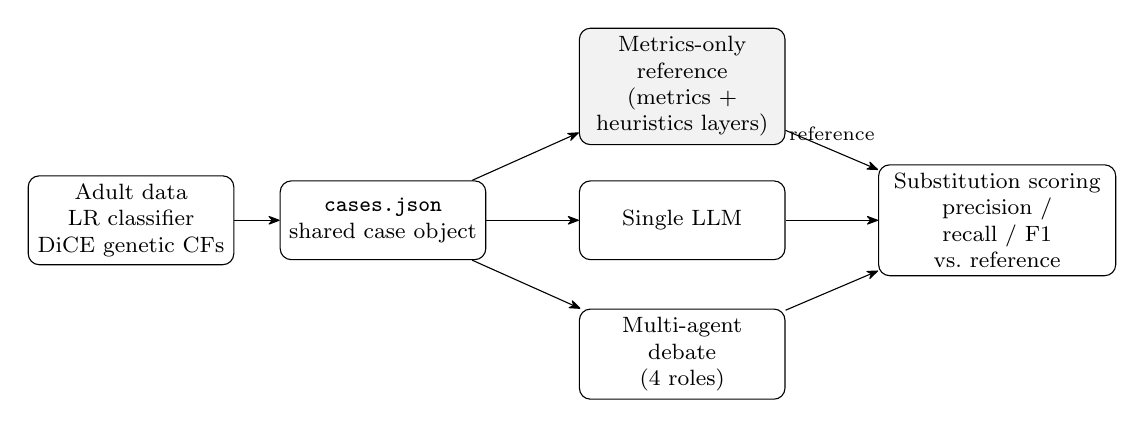
\begin{tikzpicture}[
  >={Stealth[round]},
  box/.style={draw, rounded corners, align=center, font=\footnotesize,
              inner sep=3pt, text width=24mm, minimum height=10mm},
  lay/.style={box, fill=black!5},
]
\node[box] (ml) at (0,-1.7) {Adult data\\LR classifier\\DiCE genetic CFs};
\node[box] (bridge) at (3.2,-1.7) {\texttt{cases.json}\\shared case object};
\node[lay] (ref) at (7.0,0) {Metrics-only reference\\(metrics + heuristics layers)};
\node[box] (single) at (7.0,-1.7) {Single LLM};
\node[box] (multi) at (7.0,-3.4) {Multi-agent debate\\(4 roles)};
\node[box, text width=28mm] (score) at (11.0,-1.7) {Substitution scoring\\precision / recall / F1\\vs.\ reference};
\draw[->] (ml) -- (bridge);
\draw[->] (bridge) -- (ref);
\draw[->] (bridge) -- (single);
\draw[->] (bridge) -- (multi);
\draw[->] (ref) -- node[above, font=\scriptsize] {reference} (score);
\draw[->] (single) -- (score);
\draw[->] (multi) -- (score);
\end{tikzpicture}
\caption{Pipeline. The ML stage (Logistic Regression $+$ DiCE genetic counterfactuals) is bridged into one shared \texttt{cases.json} object that feeds three evaluators. The metrics-only evaluator fuses a quantitative \emph{metrics layer} and a policy-driven \emph{heuristics layer} and serves as the Phase 2 \emph{reference}; the single LLM and the multi-agent debate are scored against it by substitution.}
\label{fig:pipeline}
\end{figure*}

\section{Pipeline and Method}
\paragraph{Dataset and classifier.}
We use the Adult Income dataset (48{,}842 rows, binary target $>$\$50K). A scikit-learn pipeline stores preprocessing --- median/most-frequent imputation, standardisation, and one-hot encoding --- together with a Logistic Regression classifier, so the identical transformation is applied at training and generation time. We deliberately keep Logistic Regression over a stronger tree ensemble: DiCE's gradient and genetic optimisers integrate cleanly with a differentiable scikit-learn pipeline, and the redundant categorical \texttt{education} column is dropped from training in favour of the ordinal \texttt{education-num}. The model reaches 0.852 accuracy / 0.656 F1 on a stratified held-out split --- adequate, since the goal is evaluating explanations, not maximising classification.

\paragraph{Counterfactual generation.}
We sample ten individuals with unfavourable predictions and ask DiCE (genetic method) for four counterfactuals each toward the favourable class, following an explicit recourse policy rather than DiCE defaults. Mutable features are \texttt{age}, \texttt{education-num}, \texttt{workclass}, \texttt{occupation}, \texttt{hours-per-week}, \texttt{capital-gain}, and \texttt{capital-loss}; \texttt{fnlwgt}, marital status, relationship, race, sex, and native country are frozen, and \texttt{education} is re-synchronised from \texttt{education-num} after generation as a display label. Each instance receives an empirical per-instance \texttt{permitted\_range}, and the genetic weights are fixed (proximity 0.2, sparsity 0.2, diversity 5.0, categorical penalty 0.1, stopping threshold 0.5) so the generator is held constant across all evaluation experiments.

\paragraph{Two deterministic layers.}
A bridge layer compiles each generated set into a compact \texttt{cases.json} object --- original instance, prediction confidence, the counterfactual array, and two kinds of precomputed evidence --- consumed identically by all evaluators. The \emph{metrics layer} reports the quantitative DiCE measures that describe the set geometrically: validity, MAD-normalised proximity (median-absolute-deviation scaling, so a \$3000 capital change and a 10-year age change are comparable), sparsity, and diversity. The \emph{heuristics layer} reports semantic recourse problems as five scored issue labels, computed from explicit thresholds (Table~\ref{tab:heuristics}) rather than left to a model to infer. Three evidence categories are kept strictly separate: the scored labels; \emph{constraint violations} (frozen-feature or out-of-range edits, treated as pipeline faults); and \emph{metric warnings} (e.g.\ \texttt{low\_count\_diversity}, derived from the metrics layer). Only the scored labels enter substitution scoring; conflating the three was an explicit design pitfall we avoided.

\begin{table}[t]
\centering
\scriptsize
\setlength{\tabcolsep}{4pt}
\caption{The heuristics layer: the five scored issue labels and the deterministic conditions that fire them. Constraint violations and metric warnings are tracked separately and are \emph{not} scored.}
\label{tab:heuristics}
\renewcommand{\arraystretch}{1.1}
\begin{tabular}{@{}p{1.02in}p{1.22in}@{}}
\toprule
Issue label & Fires when \\
\midrule
\texttt{implausible\_}\newline\texttt{time\_dependent\_}\newline\texttt{change} & age/education decreases or is non-integer; age jump $>$8\,y; education jump $>$4 levels; or education rises faster than age \\
\texttt{extreme\_}\newline\texttt{working\_hours} & hours change $\le\!-10$ or $\ge\!+15$, or result $\le$20 or $\ge$60 \\
\texttt{unactionable\_}\newline\texttt{capital\_shift} & capital-gain/loss change $\ge$\$3000 \\
\texttt{too\_many\_}\newline\texttt{changes} & $\ge$3 actionable features change (coupled work/edu pairs count once) \\
\texttt{fragile\_}\newline\texttt{counterfactual} & \texttt{cf\_confidence} $\in[0.5,0.6)$ \\
\bottomrule
\end{tabular}
\end{table}

\paragraph{The reference verdict.}
The metrics-only evaluator turns this evidence into one verdict per case via fixed rules: starting from the case-level union of flagged labels, it maps severity (any constraint violation or $\ge$2 critical issues $\rightarrow$ high; exactly one critical issue $\rightarrow$ medium; otherwise low), an assessment (\texttt{fair}/\texttt{ambiguous}/\texttt{unfair}), and an action (\texttt{accept}/\texttt{review}/\texttt{reject}). All three evaluators emit the \emph{same} verdict schema, which is what makes them directly comparable:
{\footnotesize
\begin{verbatim}
{ "case_id": 7,
  "overall_assessment": "unfair",
  "flagged_issues": ["fragile_counterfactual",
     "implausible_time_dependent_change",
     "too_many_changes"],
  "severity": "high", "confidence": 0.78,
  "recommended_action": "review" }
\end{verbatim}}
\noindent The LLM Judge appends \texttt{VERDICT\_COMPLETE} as a stop token; the optional explanation layer adds an \texttt{expert\_explanation} string. In Phase 2 the metrics-only verdict is the reference system for substitution scoring --- reference because it is reproducible and auditable, not because it is an external oracle.

\paragraph{LLM evaluators.}
Two LLM reviewers run on Groq's \texttt{llama-3.1-8b-instant}. The single evaluator reads the same case object and emits the schema above. The multi-agent debate uses four roles over a shared AutoGen \texttt{SelectorGroupChat} transcript: Prosecutor (attacks the set), Defense (defends it), Expert Witness (reads the \emph{real} DiCE metrics and never invents numbers), and Judge (synthesises the final verdict). Human reference labels are stripped from every prompt to prevent leakage. Phase 2 calibrates the single evaluator with an explicit substitution frame: start from \texttt{heuristic\_summary.flagged\_issues\_union}, keep each candidate unless the case evidence contradicts it, never add a label absent from all heuristic flags, and specifically never drop \texttt{fragile\_counterfactual} merely because a more severe issue is present. A separate, toggleable explainability layer then makes a \emph{second} LLM call that explains the already-fixed verdict in 120--180 words for non-experts; it cannot alter any label, severity, assessment, or action. A single-pass design that emitted verdict and explanation together was tested and rejected: on a case-7 smoke test the added explanation burden caused the model to silently drop \texttt{fragile\_counterfactual} from the verdict.

\paragraph{Agreement metrics.}
We treat each issue label the reference flags as the positive class and report the standard precision/recall/F1 vocabulary, so substitution scoring and ground-truth scoring use one set of names. \emph{Recall} is the fraction of reference issue labels the system also flags (previously called ``detection rate''); \emph{precision} is the fraction of system-flagged labels the reference also flags; \emph{F1} is their harmonic mean; and \emph{exact-match rate} is the fraction of cases whose issue set is identical to the reference. We also report \emph{assessment/severity/action agreement} --- the fraction of cases with an identical scalar \texttt{overall\_assessment}, \texttt{severity}, or \texttt{recommended\_action}.

\paragraph{Setup and cost.}
All LLM runs use \texttt{llama-3.1-8b-instant} at temperature 0.2. Groq's free tier costs nothing but caps throughput (30 requests/min, 6K tokens/min, 14.4K requests/day), so runs insert ${\sim}70$\,s delays between calls and between cases; the debate additionally had to be capped at one specialist round and 250 completion tokens after a Judge request hit 6005 tokens against the 6000-token ceiling. The cost columns are therefore \emph{estimates} --- token counts $\times$ Groq's published per-token price --- indicating relative compute rather than money actually spent, which was zero.

\section{Experiments and Results}
\paragraph{Phase 1: comparing architectures.}
Table~\ref{tab:systems} reports the three architectures scored against the team-drafted reference. This stage exercised the whole system end to end --- prompt safety, transcript saving, verdict parsing, and quota-safe orchestration. The headline result is uncomfortable: the fully deterministic baseline leads on recall (88.9\%) and precision (96.0\%), and the multi-agent debate is worst on every metric (recall 66.7\%, exact match 0\%) at roughly double the per-case cost. The debate's failures were diagnostic, not random. It \emph{over-flagged} the semantic label \texttt{inconsistent\_work\_profile} --- predicting it in 9 of 10 cases though the reference contained it in only 3, which is precisely why its precision collapses to 54.6\% --- and \emph{under-detected} \texttt{fragile\_counterfactual}, dropping it even though the flag was present in the heuristic evidence the Judge received. A confound points away from the architecture itself: debate prompts run 13--16K tokens against ${\sim}3$--4K for the single LLM on the \emph{same} 8B model, so the gap is consistent with the small model losing coherence in long context. Two decisions followed: we removed \texttt{inconsistent\_work\_profile} from the scored taxonomy (its heuristic almost never fired while LLMs over-applied it, leaving five labels), and we reframed the closeout experiment around substitution.

\begin{table}[t]
\centering
\scriptsize
\setlength{\tabcolsep}{5pt}
\caption{Phase 1: agreement of the three evaluators with the team-drafted reference labels (label-level \%, with exact issue-set match). Calls per case: metrics-only 0, single LLM 1, debate 4+.}
\label{tab:systems}
\begin{tabular}{@{}lrrrr@{}}
\toprule
System & Prec & Recall & F1 & Exact \\
\midrule
Metrics-only & 96.0 & 88.9 & 92.3 & 60 \\
Single LLM & 95.7 & 81.5 & 88.0 & 60 \\
Multi-agent debate & 54.6 & 66.7 & 60.0 & 0 \\
\bottomrule
\end{tabular}
\end{table}

\paragraph{Methodology pivot.}
A second problem is that the draft labels were authored by the same team that wrote the heuristics --- the file itself is marked an ``initial human-perspective draft for team review'' --- so any agreement between heuristic coverage and the labels is partly circular. We therefore stop presenting them as independent truth. Phase 2 makes the deterministic metrics-only evaluator the reference system and measures how closely an LLM approximates it, and what interpretive value it adds.

\begin{table}[t]
\centering
\scriptsize
\setlength{\tabcolsep}{4pt}
\caption{Phase 2: substitution against the metrics-only reference (label-level \%, plus estimated USD/case). Scalar assessment agreement stays at 50\% throughout.}
\label{tab:phase2}
\begin{tabular}{@{}lrrrrr@{}}
\toprule
System & Prec & Recall & F1 & Exact & Cost \\
\midrule
Uncalibrated single LLM & 100 & 84 & 91.3 & 60 & .00029 \\
Calibrated single LLM & 100 & 96 & 98.0 & 90 & .00030 \\
Calibrated $+$ explanation & 96 & 96 & 96.0 & 80 & .00050 \\
\bottomrule
\end{tabular}
\end{table}

\paragraph{Phase 2: calibration.}
Prompt calibration produced the main quantitative gain (Table~\ref{tab:phase2}): recall rose from 84\% to 96\% and exact issue-set match from 60\% to 90\%, with precision held at 100\% (no extra labels introduced). The gain concentrated exactly where the uncalibrated model was failing --- the silently dropped \texttt{fragile\_counterfactual}. Case 7 is illustrative: two of its counterfactuals have \texttt{cf\_confidence} $\approx 0.548$ and $0.553$, just inside the $[0.5,0.6)$ fragility band, and the calibrated model recovered the label to reach an exact match where the uncalibrated run had missed it. One disagreement persists (case 0), which we keep rather than hide: even explicit calibration does not guarantee substitution, because the model still tends to prioritise the most semantically salient issues over a low-severity robustness label. This supports treating each disagreement as a site for inspection --- the LLM may have erred, but a rule may also be too rigid.

\paragraph{Phase 2: explainability.}
The explainability run preserved 96\% recall, but precision dipped to 96\% (one extra label) and exact match fell to 80\%. This is not the explanation step editing a verdict --- the explanation is generated \emph{after} the verdict is fixed --- but ordinary stochastic variance in a fresh run, concentrated on two boundary cases. Its value is qualitative: the \texttt{expert\_explanation} field turns terse labels into a readable account of why a set is fragile, implausible, or over-burdensome, at ${\sim}67\%$ higher estimated cost per case. Notably, scalar agreement stayed near 50\% across all runs: matching the issue \emph{set} is easier than matching the reference's full severity/assessment/action policy, because the 8B model gravitates to a harsher qualitative judgement once any issue is present.

\section{Discussion}
Three conclusions follow. First, deterministic evaluation is the right backbone here: it is free after setup, reproducible, auditable, and directly tied to the recourse policy, and it forces the evaluation's assumptions into the open --- which features are mutable, which causal changes are accepted, and which signals are merely metric-level warnings rather than scored issues. Second, the LLM is useful precisely when its role is constrained. Unconstrained, it under-detects fragile cases and invents semantic labels (the Phase-1 debate); calibrated to start from the heuristic union and forbidden to add unsupported labels, a single 8B model substitutes the reference issue set closely (96\% recall, 90\% exact match) while contributing a natural-language rationale. This is a clean division of labour: rules define the evidence surface, the LLM interprets and communicates it. Third, more agents are not automatically better. The adversarial debate enriched the project technically --- role orchestration, transcript analysis, judge parsing --- but empirically over-flagged and under-detected under the small-model, quota-safe setting. At this scale the calibrated single LLM is the stronger LLM-based evaluator, and the persistent ${\sim}50\%$ scalar agreement shows that even it does not yet substitute the reference's full severity/action policy.

\section{Limitations and Reproducibility}
The study is intentionally small: one dataset, one classifier family, ten sampled unfavourable cases, and one main 8B Groq model. The deterministic reference is a designed artifact encoding our policy choices, not an external adjudicated benchmark, and the calibration confound (model size vs.\ architecture) was diagnosed but not fully isolated --- testing a 70B model on the debate is the obvious next step. A stronger study would add independent human re-annotation with inter-annotator agreement, more datasets, larger models, and a sensitivity analysis over the heuristic thresholds of Table~\ref{tab:heuristics}. The GitHub repository contains the code, walkthrough documentation, scripts, and result artifacts needed to reproduce every number above: \url{https://github.com/Teytey2002/Multi-Agent_AdversarialEvaluationofCounterfactualExplanations}.

\section{Conclusion}
We built and evaluated an end-to-end pipeline for assessing DiCE counterfactual explanations beyond standard numerical metrics, comparing a deterministic heuristic reference, a single LLM, and a multi-agent debate over one shared case representation. The finding is pragmatic: deterministic heuristics are the most reliable backbone, a calibrated single LLM can approximate that reference and add readable explanations at negligible cost, and the multi-agent debate is a documented negative result --- more agents did not yield better evaluation at this scale. The closeout system therefore combines structured recourse rules, substitution scoring, and an optional LLM explanation layer as a compact and defensible approach for a course-scale counterfactual evaluation study.

\bibliography{references}

\end{document}
